% 文档类型
\documentclass[a4paper, 12pt]{article} % options: {book, }
% 标题信息
\title{\emph{\LaTeX} 自查手册} % 标题
\author{Xiong Lingyu} % 作者
\date{\today} % 日期

% 加载宏包
\usepackage{ctex} % 中文包
\usepackage{fontspec} % 字体包
% 设置字体(默认使用宋体)
% \setCJKmainfont{SimSun}   % 宋体
% \setCJKmainfont{FangSong} % 仿宋
% \setCJKmainfont{NSimSun}  % 新宋体
%\setCJKmainfont{STFangsong} % 华文仿宋
%\setCJKmainfont{STZhongsong}% 华文中宋
%\setCJKmainfont{STXihei}  % 华文细黑
%\setCJKmainfont{KaiTi}    % 楷体
%\setCJKmainfont{STKaiti}  % 华文楷体
%\setCJKmainfont{SimHei}   % 黑体
% \setCJKmainfont{Microsoft YaHei}  % 微软雅黑
%\setCJKmainfont{LiSu}     % 隶书
%\setCJKmainfont{STLiti}   % 华文隶书
%\setCJKmainfont{YouYuan}  % 幼圆
\usepackage{geometry} %
\geometry{left=2cm, right=2cm, top=2cm, bottom=2cm}

\usepackage{amsmath} % 公式包
\usepackage{mathrsfs} % 公式字体包
\usepackage{amssymb} % 公式字体包
\numberwithin{equation}{section} % 让公式编号带上章节
\numberwithin{figure}{section} % 让图表带上章节 

\usepackage{multicol} % 多栏环境
\columnseprule 1pt % 设置分栏线
\columnsep 1cm % 设置栏间隔
\usepackage{graphicx} % 插入图片包
\usepackage{hyperref} % 提供引用链接,包括文内和文外
\hypersetup{hidelinks, colorlinks=true, linkcolor=blue} % 链接配置

\usepackage{float} % 排版图片位置包


\usepackage{fancyhdr} % 页眉页脚包
\pagestyle{fancy}  % 设置页眉页脚格式
\setlength{\headheight}{15pt}
\lhead{} \chead{LaTex 自查手册} \rhead{}

\usepackage{blindtext} % 随机文字
\usepackage{draftwatermark}
\usepackage{everypage}
\SetWatermarkText{Xiong Lingyu}
% \SetWatermarkLightness {0}
% \SetWatermarkAngle {45}
% \SetWatermarkColor{gray}
\SetWatermarkScale {0.5}



\allowdisplaybreaks % 允许公式跨页
\linespread{1.25} % 设置文本行距
\begin{document}
    \maketitle

    \newpage % 增加空白页
    {\centering\tableofcontents}
    \setcounter{tocdepth}{1}
    \newpage
    % 为章节添加标签便于引用
    
    \section{引言} \label{sec:intro} 
    引言是文章的第一部分,主要包含作者对研究背景的调查、文献调研综述、文章主要特色以及章节安排。
    %引用章节
    我们在 章节 \ref{sec:method} 中详细叙述了使用的方法  
    % 为公式添加标签便于引用
    \section{方法} \label{sec:method} 
    这一章主要是作者提出的新方法,并论述其主要特点以及证明等。
        \subsection{方法一} \label{subsec:method1}
            允许公式跨页:\verb|\allowdisplaybreaks| 
            \begin{equation} \label{eq:sum}
                f(x) = \sum_{i=0}^{x-1} f(i)
            \end{equation}
            % 引用公式
            公式 \ref{eq:sum} 详细说明了函数 $f(x)$。 
            % 不带编号的公式
            \begin{equation*} 
                f(x) = x^3 + x^2 + x
            \end{equation*}
            另一个公式:合并公式编号
            \begin{equation} \label{eq:align}
                \begin{split}  % 使用 split 将多行公式合并成一个编号
                &\ x^4+2x^3+11x^2+18x+18 \\
                &=\ (x^2+2x+2)(x^2+9) \\
                &=\ (x^2+x+3)^2+(2x+3)^2
                \end{split}
                \end{equation}
            下一个公式:取消某行编号
            \begin{align}
                f(x) &= (x+1)^2 \nonumber \\  % 使用 \nonumber 取消编号
                &= x^2 + 2x + 1
            \end{align}
            下一个公式:全部居中对齐
            \begin{gather} % 默认全部居中对齐
                \boxed{   % \boxed 给公式加框
                    \begin{split}
                        2x + 3 = 5678y - 8765z + 20 \\
                        6x = y + z + 555666
                    \end{split}
                }
            \end{gather}
            下一个公式:分段函数或联立方程
            \begin{align}
                \text{ReLU}(x) = 
                \begin{cases}
                    x \quad\text{if } x > 0 \\
                    0 \quad\text{otherwise}
                \end{cases}
            \end{align}
            下一个公式:\verb|\mathrm{}| 将公式中斜体字母改为正体
            \begin{equation}
                \mathrm{e}^{\mathrm{i}\theta} = \cos\theta + \mathrm{i}\sin\theta
            \end{equation}
            矩阵一: `pmatrix';矩阵二:`bmatrix';矩阵三:`vmatrix';矩阵四:`Bmatrix'。
            \begin{equation}
                \begin{pmatrix}
                    a_{11} & \cdots & a_{1n} \\
                    a_{21} & \cdots & a_{2n} \\
                    \vdots & \ddots & \vdots \\
                    a_{n1} & \cdots & a_{nn} \\
                \end{pmatrix}
                \begin{bmatrix}
                    a_{11} & \cdots & a_{1n} \\
                    a_{21} & \cdots & a_{2n} \\
                    \vdots & \ddots & \vdots \\
                    a_{n1} & \cdots & a_{nn} \\
                \end{bmatrix}
                \begin{vmatrix}
                    a_{11} & \cdots & a_{1n} \\
                    a_{21} & \cdots & a_{2n} \\
                    \vdots & \ddots & \vdots \\
                    a_{n1} & \cdots & a_{nn} \\
                \end{vmatrix}
                \begin{Bmatrix}
                    a_{11} & \cdots & a_{1n} \\
                    a_{21} & \cdots & a_{2n} \\
                    \vdots & \ddots & \vdots \\
                    a_{n1} & \cdots & a_{nn} \\
                \end{Bmatrix}
            \end{equation}
        \subsection{方法二} \label{subsec:method2}
            \begin{itemize}
                \item \verb|\newcommand{}{}|:使用类似于 C 语言中的宏替换命令,可以将一些长的命令用短的命令替换。
                \item \verb|\newcommand{}{}|:使用类似于 C 语言中的宏替换命令,可以将一些长的命令用短的命令替换。
                \item 添加页眉和页脚:\verb|\usepackage{fancyhdr} \pagestyle{fancy} \lhead{} \lfoot{}|。
                \item 添加水印:\verb|\usepackage{draftwatermark} \usepackage{everypage}|。
                \item 添加脚注:\verb|\footnote{}|。这是一个脚注\footnote{添加的脚注}
                \item 目录:\verb|\tableofcontents|
                \item 行距:\verb|\linespread{}|
                \item 修改字体:\verb|\usepackage{fontspec}|
                \item 部分:\verb|\part{}|;章:\verb|\chapter{}|;节:\verb|\section{}|;小节:\verb|\subsection{}|。
                \item 带编号列表:使用 \verb|\begin{enumerate}|。
                    \begin{enumerate}
                        \item 第一条
                        \item 第二条
                    \end{enumerate}
                \item 空格:窄空格:\verb|\,|空\,格;中等空格:\verb|\:|空\:格;宽空格:\verb|\;|空\;格;词见空格:\verb|\ |空\ 格。
                \item 设置页边距:\verb|\usepackage{geometry}|
                \item 英文字母几种变体效果:
                    \begin{enumerate}
                        \item \verb|\mathcal{}| $\mathcal{ABCBEFG}$
                        \item \verb|\mathscr{}(需\usepackage{mathrsfs})| $\mathscr{ABCBEFG}$
                        \item \verb|\mathbb{}(需\usepackage{amssymb})| $\mathbb{ABCBEFG}$
                        \item \verb|\mathfrak{}(需\usepackage{amssymb})| $\mathfrak{ABCDEFG}$
                        \item \verb|\mathsf{}| $\mathsf{ABCDEFG}$
                        \item \verb|\mathbb{}| $\mathbf{ABCDEFG}$
                    \end{enumerate}
                \item 多栏环境:\verb|\usepackage{multicol} \begin{multicols}| \begin{multicols}{2}
                    [这是在多栏环境中添加单栏文字;这是在多栏环境中添加单栏文字]
                    多栏环境多多栏环境多栏环境多栏环境多栏环境多栏环境多栏环境多栏环境多栏环境多栏环境多栏环境多栏环境多栏环境多栏环境多栏环境多栏环境多栏环境多栏环境多栏环境多栏环境多栏环境多栏环境多栏环境多栏环境多栏环境多栏环境。
                \end{multicols}
            \end{itemize}
            
        \subsection{方法三} \label{subsec:method3}
            有四种宽度: 
            \verb|\paperwidth| \quad 
            \verb|\textwidth| \quad
            \verb|\linewidth| \quad
            \verb|\columnwidth|
            \begin{figure}[H] % 强制按照文章书写顺序排版图片
                \centering
                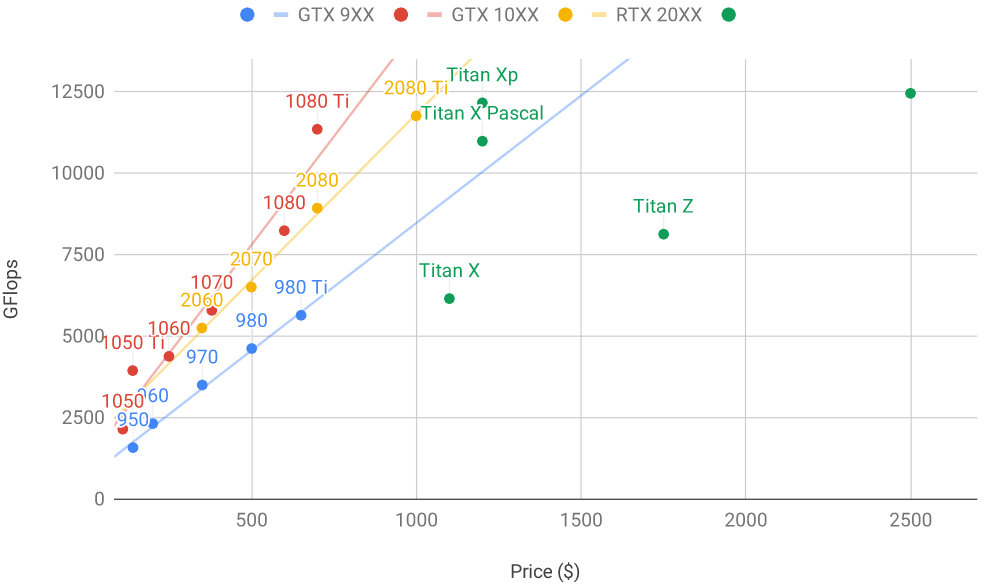
\includegraphics[width=0.9\linewidth]{img/GPU-flops-vs-price.png}
                \caption{\label{figure:gpu} GPU vs Price}
            \end{figure}
            图 \ref{figure:gpu} 展示了,,,。
    \section{实验或仿真结果} \label{sec:experiment}
    这一章针对提出的方法有效性进行实验验证,并通过对比或消融实验验证改进点的有效性。
    \section{结论} \label{sec:conclusion}
    对全文进行总结,主要叙述文章的创新点,解决了哪些问题,方法提升到了什么程度,并适度进行展望\cite{einstein,knuthwebsite,latexcompanion}。
    \addcontentsline{toc}{section}{参考文献}
    \bibliographystyle{plain}
    \bibliography{refs}
\end{document}